\documentclass{beamer}

\mode<presentation>
{
  \usetheme{CambridgeUS}      % or try Darmstadt, Madrid, Warsaw, ...
  \usecolortheme{default} % or try albatross, beaver, crane, ...
  \usefonttheme{default}  % or try serif, structurebold, ...
  \setbeamertemplate{navigation symbols}{}
  \setbeamertemplate{caption}[numbered]
} 

\usepackage[spanish]{babel}
\usepackage[utf8x]{inputenc}
\usepackage{tensor}
\usepackage{amssymb}
\usepackage{amsmath}
\usepackage{float}
\usepackage{movie15}

\graphicspath{ {./imagenes/} }

\title[Creación y aniquilaci\'on de part\'iculas]{Creaci\'on y aniquilaci\'on de part\'iculas}

\author{Particuleros}

\institute{\bf Universidad de Sonora}
%\textsc {Industrial Training Presentation }

\date{22 de mayo de 2019}

\begin{document}

\begin{frame}
\begin{figure}
    \centering
    
\includegraphics[scale=.35]{logoo.png}
    
    
\end{figure}
  \titlepage
\end{frame}


\section{Índice}

\begin{frame}{Índice}

\begin{itemize}
  \item Origen histórico.
  \begin{itemize}
      \item Positrón y Antimateria.
      
  \end{itemize}
  
  \item Creación de pares.
  \begin{itemize}
      \item Conceptos clave.
      \item Condiciones para la creación de pares.
      \item Principio de incertidumbre de Heisemberg.
      \item Justificación matemática.
  \end{itemize}
  \item Aniquilación partícula-antipartícula.
  \begin{itemize}
      \item Part\'icula-Antipart\'icula.
      \item Electrón-Positrón.
    %   \begin{itemize}
    %       \item Caso de Alatas energ\'ias
    %       \item Caso de Bajas energ\'ias
    %   \end{itemize}
      \item Protón-antineutrón.
    %  \item Producción de Higgs.
  \end{itemize}
    \item Radiación de Hawking.
  \begin{itemize}
      \item Descripci\'on
      \item Temperatura de la radiación del agujero negro
  \end{itemize}
   \item Conclusión
        \begin{itemize}
            \item Aplicaciones
            \item Problema
        \end{itemize}
\end{itemize}

% Commands to include a figure:
% \begin{figure}
% 
\includegraphics[width=5cm ,height= 3cm]{oltas-header.jpg}
% \caption{\label{fig:your-figure}OLTAS}
% \end{figure}
% \vskip 1cm

\end{frame}
%%%%%%%%%%%%%%%
\section{Origen histórico.}

\begin{frame}{Positrón y antimateria.}
\begin{figure}
    \centering
    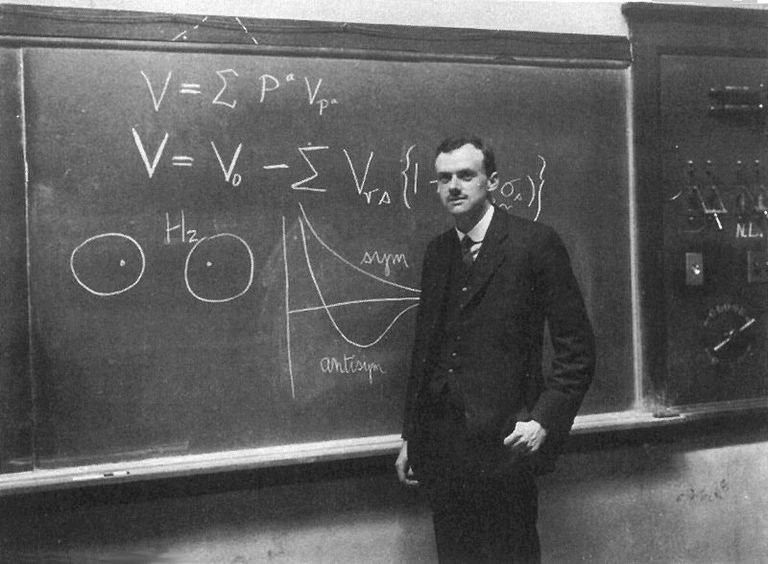
\includegraphics[scale=.25]{dirac.jpg}
    \caption{Paul Dirac; responsable de la predicción de la partícula llamada \textit{positrón}, dando luz verde a futuras investigaciones sobre creación y aniquiliación de partículas.}
    \label{fig:dirac}
\end{figure}


\end{frame}

%%%%%%%%%%%%%%%%%%%%%%%%%%%%%%%%%%%%%%%%%%%%%%%%
\section{Origen histórico.}

\begin{frame}{Positrón y antimateria.}
\begin{figure}
    \centering
    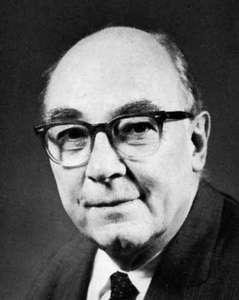
\includegraphics[scale=.45]{anderson.jpg}
    \caption{Carl D. Anderson; fue el primer científico en mostrar el positrón en un experimento.}
    \label{fig:anderson}
\end{figure}


\end{frame}
%%%%%%%%%%%%%%%%%%%%%%%%%%%%%%%%%%%%%%%%%%%%%%%%%%%%%%%%%%%%%%%%%%%%%%%%%%%
\section{Origen histórico.}

\begin{frame}{Positrón y antimateria.}
\begin{figure}
    \centering
    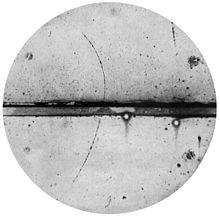
\includegraphics[scale=.60]{positron.jpg}
    \caption{Representación experimental del positrón, en base a las primeras aproximaciones dadas por Paul Dirac.}
    \label{fig:positron}
\end{figure}


\end{frame}
%%%%%%%%%%%%%%%%%%%%%%%%%%%%%%%%%%%%%%%%%%%%%%%%%%%%%%%%%%%
\section{Origen histórico.}

\begin{frame}{Positrón y antimateria.}
\begin{figure}
    \centering
    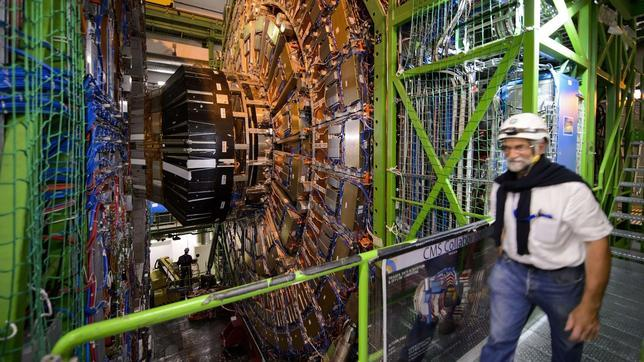
\includegraphics[scale=.50]{lhc.jpg}
    \caption{Gran Colisionador de Hadrones en el año 1990.}
    \label{fig:positron}
\end{figure}


\end{frame}
%%%%%%%%%%%%%%%%%%%%%%%%%%%%%%%%%%%%%%%%%%%%%%%%%%%%%%%%%%%%%%
\section{Creación de Pares.}

\begin{frame}{Conceptos clave.}

% \begin{itemize}
%   \item OLTAS is a part of MySpace.
%   \item MySpace is totally for customer’s space, where different types of services like insurance schemes , cheque printing, online payments, gifts and voucher offers provided by Yes Bank under one application.

% \end{itemize}

% Commands to include a figure:

Cuando un fotón tiene suficiente energía, puede crear materia en forma de un par partícula-antipartícula. Tales conversiones solo pueden tomar lugar donde no se viola la ley de conservación de la energía. En adición a la carga y a la conservación de el \textit{momento-energía}, otros números cuánticos pueden afectar a los posibles estados finales de el fotón.


\begin{figure}[h]
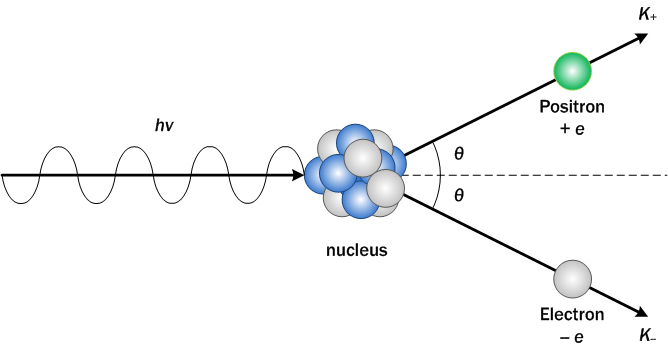
\includegraphics[scale=.18]{par1.jpg}
\caption{\label{fig:creacionpar}Representación gráfica de la creación par.}
\end{figure}

\vskip 1cm

\end{frame}

%%%%%%%%%%%%%%%
\begin{frame}{Principio de incertidumbre de Heisemberg}
    La creación de partículas en el vacío se debe a este principio el cual, a primera instancia, nos menciona que no se puede conocer la velocidad y posición exacta de una partícula debido a que mientras más conoces una más se desconoce la otra.
    \begin{equation*}
        \Delta x \Delta v = \hbar/2
    \end{equation*}
    Esto también aplica para la energía
    \begin{equation*}
        \Delta E \Delta t = \hbar/2
    \end{equation*}
\end{frame}
%%%%%%%%%%%%%%%
\begin{frame}{Condiciones para la creaci\'on de pares}
\begin{itemize}
    \item El proceso de creaci\'on de pares no puede darse en el vac\'io, pues como se demostrar\'a a continuaci\'on, es imposible que en ausencia de materia se pueda conservar la energia y el momento al mismo tiempo.
    \item El fotón debe ser lo suficientemente energético para poder \textit{generar}un par. La energía mínima que el fotón debe contener para que la creación de un par se produzca es de 1.022 $MeV$, para poder así generar el par \textit{positrón-electrón} con 0.511 $MeV$, representado como masa, cada uno de estos.
    \item Estas partículas virtuales se crean debido a las fluctuaciones cuánticas explicadas por el principio de incertidumbre de Hesienberg.
\end{itemize}
\end{frame}

%%%%%%%%%%%%%%%

%%%%%%%%%%%%%%%

\begin{frame}{Justificaci\'on matem\'atica}
    Suponemos que un fotón en el vac\'io se transforma en un par electr\'on ($P_1$) positr\'on ($P_2$) como se muestra en la \textit{figura \ref{fig:jm_cracion}}.
        
    \begin{figure}[h]
    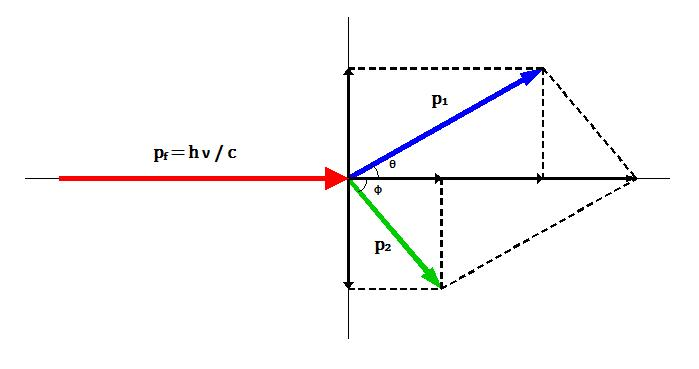
\includegraphics[scale=.40]{Dibujo_Pares.jpg}
    \caption{\label{fig:jm_cracion}Diagrama de la situaci\'on f\'isica. Un fot\'on desaparece creando un par electr\'on-positr\'on}
    \end{figure}
\end{frame}

\begin{frame}{}
    Estado inicial: El fotón viaja en direcci\'on positiva del eje x. La energ\'ia inicial y el momento del fotón son:
        \begin{equation*}
        \begin{split}
            \Vec{p}_f &= \frac{h\nu}{c} \hat{i}\\
            E_f &= h\nu
        \end{split}
        \end{equation*}
    Estado final: El fotón ha desaparecido creando un electr\'on ($1$) que se desplaza en una direcci\'on que forma un \'angulo $\theta$ hacia arriba con respecto al eje x; y un positr\'on ($2$) que se desplaza en una direcci\'on que forma un \'angulo $\phi$ hacia abajo con respecto al eje x. Sus momentos y energ\'ias son:
        \begin{equation*}
        \begin{split}
            \Vec{p}_1 &= p_1\cos{\theta} \hat{i} + p_1\sin{\theta}\hat{j}\\
            \Vec{p}_2 &= p_2\cos{\phi} \hat{i} - p_2\sin{\phi}\hat{j}\\
            E_1 &= \sqrt{m^2c^4 + p^2_1c^2}\\
            E_2 &= \sqrt{m^2c^4 + p^2_2c^2}
        \end{split}
        \end{equation*}
\end{frame}

\begin{frame}{}
    De la conservaci\'on del momento:
    \begin{equation}
        \Vec{p}_f = \Vec{p}_1 + \Vec{p}_2
    \end{equation}
    \begin{equation}
        \frac{h\nu}{c} = p_1\cos{\theta} + p_2\cos{\phi}
    \end{equation}
    Observemos que $ p_1\cos{\theta} + p_2\cos{\phi} \leq p_1 + p_2 $, entonces
    \begin{equation}\label{leq}
    \boxed{
        \frac{h\nu}{c} \leq p_1 + p_2
        }
    \end{equation}
\end{frame}{}
\begin{frame}{}
    De la conservaci\'on de la Energ\'ia:
    \begin{equation*}
        \begin{split}
            h\nu &= E_1 + E_2\\
            (h\nu)^2 &= E^2_1 + E^2_2 + 2E_1E_2\\
            (h\nu)^2 &= 2m^2c^4 + p^2_1c^2 + p^2_2c^2 + 2E_1E_2\\
            \left (\dfrac{h \ \nu}{c}\right )^2 &= 2m^2c^2 + p^2_1 + p^2_2 + \frac{2}{c^2}\sqrt{(m^2c^4 + p^2_1c^2)(m^2c^4 + p^2_2c^2)}\\
            \left (\dfrac{h \ \nu}{c}\right )^2 &= p_1^2 + p_2^2 + 2 m^2c^2 + 2\sqrt{p_1^2 p_2^2+p_1^2 m^2 c^2+p_2^2 m^2 c^2+m^4 c^4}
        \end{split}
    \end{equation*}
    En esta \'ultima igualdad todos los sumandos del interior del radicando son no negativos con $m^4c^4$ y $2m^2c^2$ mayores de cero, lo que nos permite deducir la siguiente desigualdad rigurosa:
    \begin{equation*}
        \begin{split}
            \left (\dfrac{h \ \nu}{c}\right )^2 > p_1^2 + p_2^2 + 2 m^2c^2 + 2\sqrt{p_1^2 p_2^2}
        \end{split}
    \end{equation*}
\end{frame}{}
\begin{frame}{}
        \begin{equation*}
        \begin{split}
            \left (\dfrac{h \ \nu}{c}\right )^2 > p_1^2 + p_2^2 + 2 \ p_1 \ p_2 = (p_1 + p_2)^2
        \end{split}
    \end{equation*}
    Entonces
        \begin{equation}\label{geq}
        \boxed{
        \dfrac{h \ \nu}{c} > p_1 + p_2
        }
    \end{equation}
    Podemos ver que la ecuaci\'on \eqref{leq} y \eqref{geq} presentan una inconsistencia matem\'atica por lo que queda demostrado que en el vac\'io no se pueden crear pares de part\'icula-antipart\'icula mientras se conserva la energ\'ia y el momento simultaneamente.
\end{frame}{}
%%%%%%%%%%%%%%%%%%%%%%%%%%%%%%%%%%

%meet me at the corner -  red hot chilli peppers
%%%%%%%%%%%%%%%%%%%%%%%%%%%%%%%%%%%

%por que haces la bibliografia ahi?
% quién anda ahí?
% tu gfa
% orale gfa, deme dinero
% y el putazo donde?
%%%%%%%%%%%%%%%%%%%%%%%%%%%%%%%%%%
\section{Aniquilaci\'on part\'icula-antipart\'icula}
\begin{frame}{Part\'icula-antipart\'icula}
    La aniquilaci\'on ocurre cuando una part\'icula colisiona con su respectiva antipart\'icula. La energ\'ia total y el momento del par inicial de part\'iculas se conserva en el proceso y se distribuye entre las part\'iculas del estado final.
    Esta aniquilación se debe a que cuando una se encuentra con su anti-partícula, ambas poseen la misma masa pero sus números cuánticos son opuestos, de modo que cuando interactúan estos el resultado de los número cuánticos es cero.
\end{frame}{}
%%%%%%%%%%%%%%%%%%%%%%%%%%%%%%%%%%%%
\begin{frame}{Electr\'on-Positr\'on}
    Este proceso debe satisfacer algunas leyes de conservaci\'on en las que se incluyen:
    \begin{itemize}
        \item Concervaci\'on de la carga electrica. La carga neta antes y despues es cero.
        \item Conservaci\'on del momento lineal y de la energ\'ia total. Esto prohibe la creaci\'on de un solo fot\'on.
        \item Conservaci\'on del numero total de leptones.
    \end{itemize}
    \begin{figure}[h]
        \centering
        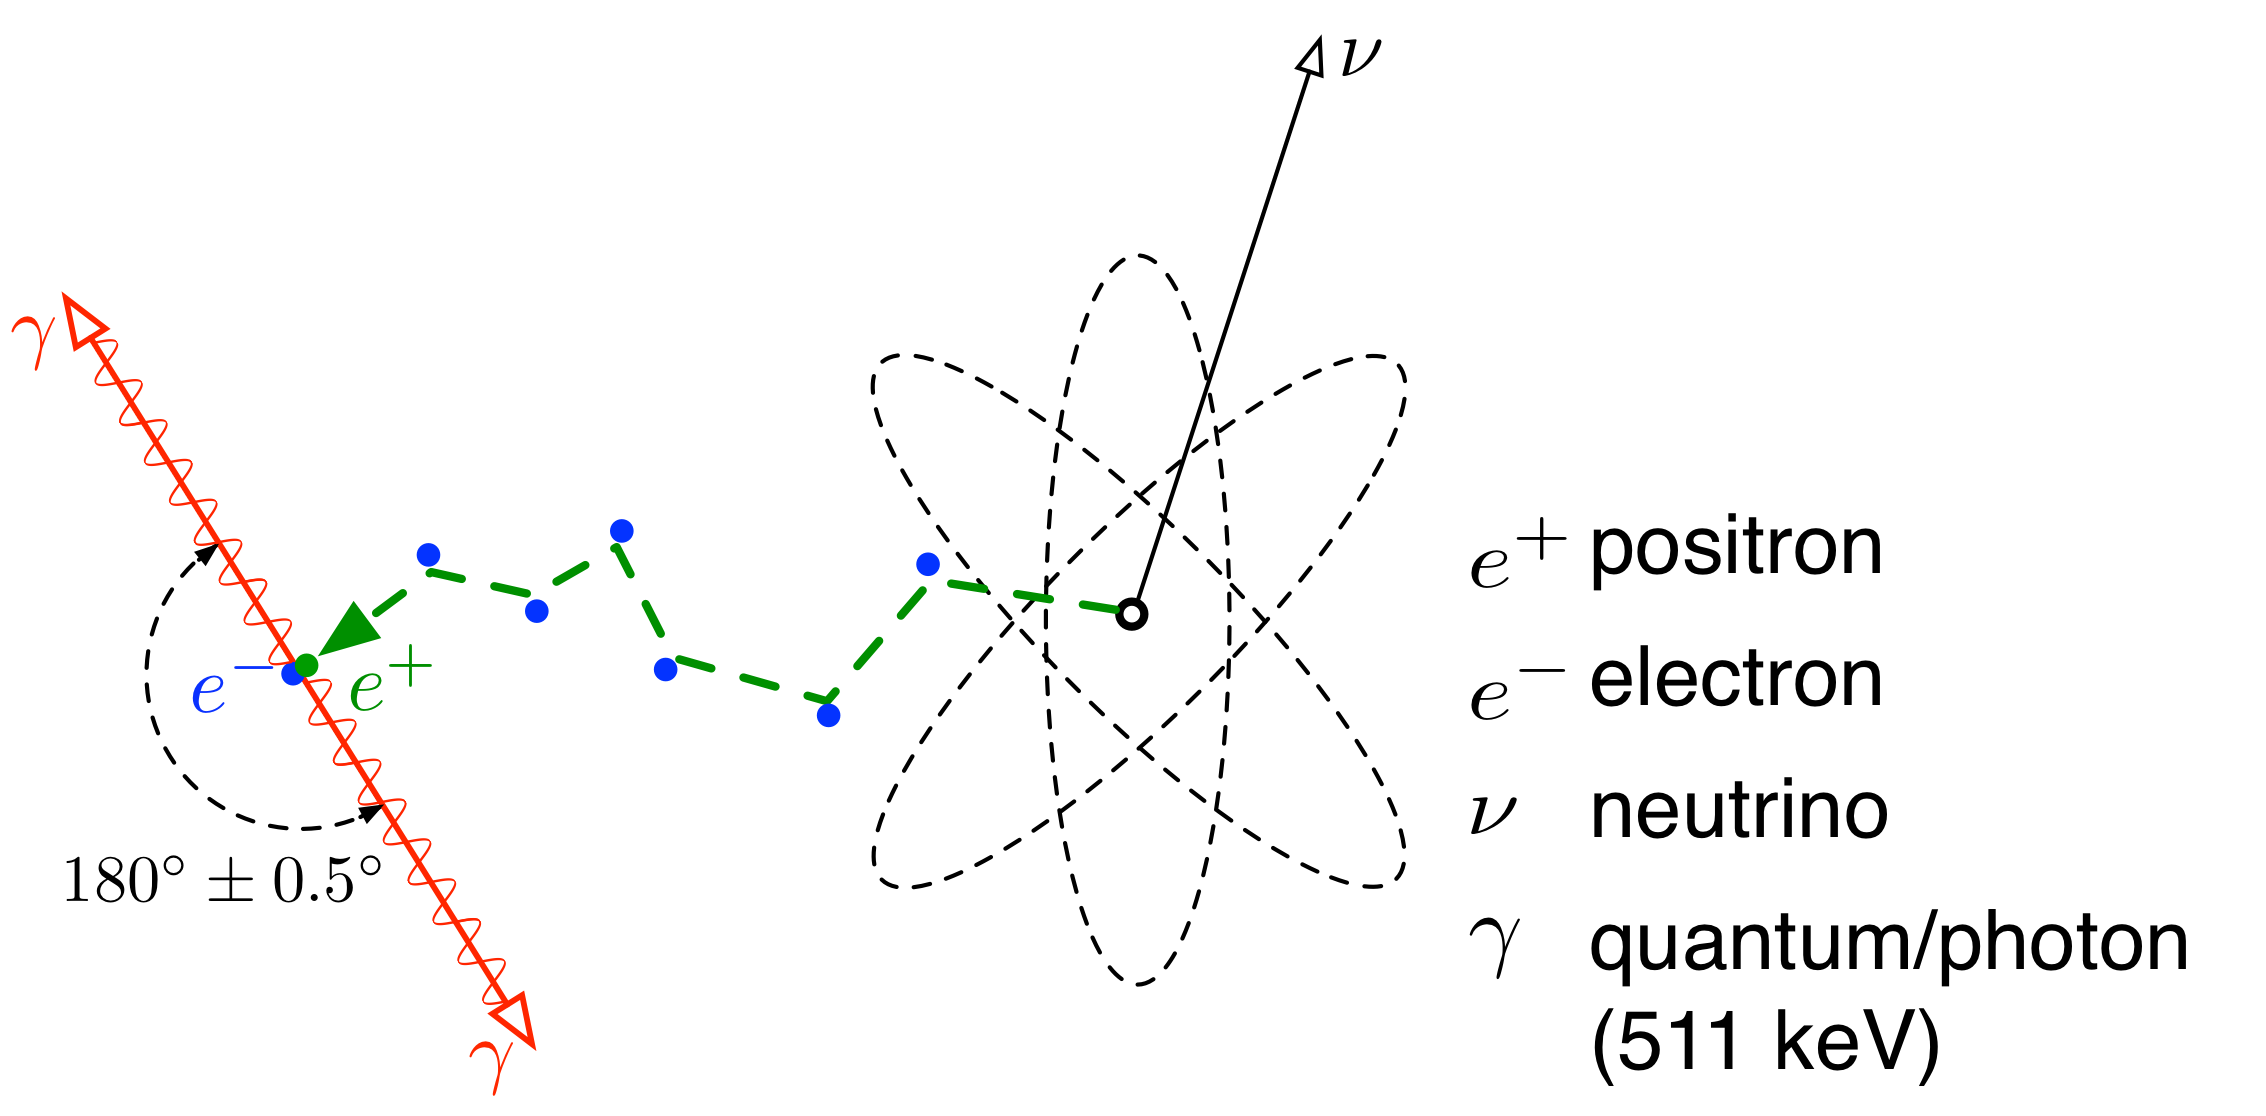
\includegraphics[scale = 0.6]{aniquilacion-par.png}
        \caption{Aniquilaci\'on de un electr\'on proveniente del decaimiento beta con un positr\'on.}
        \label{fig:A-natural}
    \end{figure}

\end{frame}
%%%%%%%%%%%%%%%%%%%%%%%%%%%%%%%%%

\begin{frame}{Colisi\'on a bajas energ\'ias}
        A bajas energias, el resultado de la colisi\'on es la aniquilaci\'on del electr\'on y positr\'on y la creaci\'on de dos fotones.
        
        \begin{figure}
            \centering
            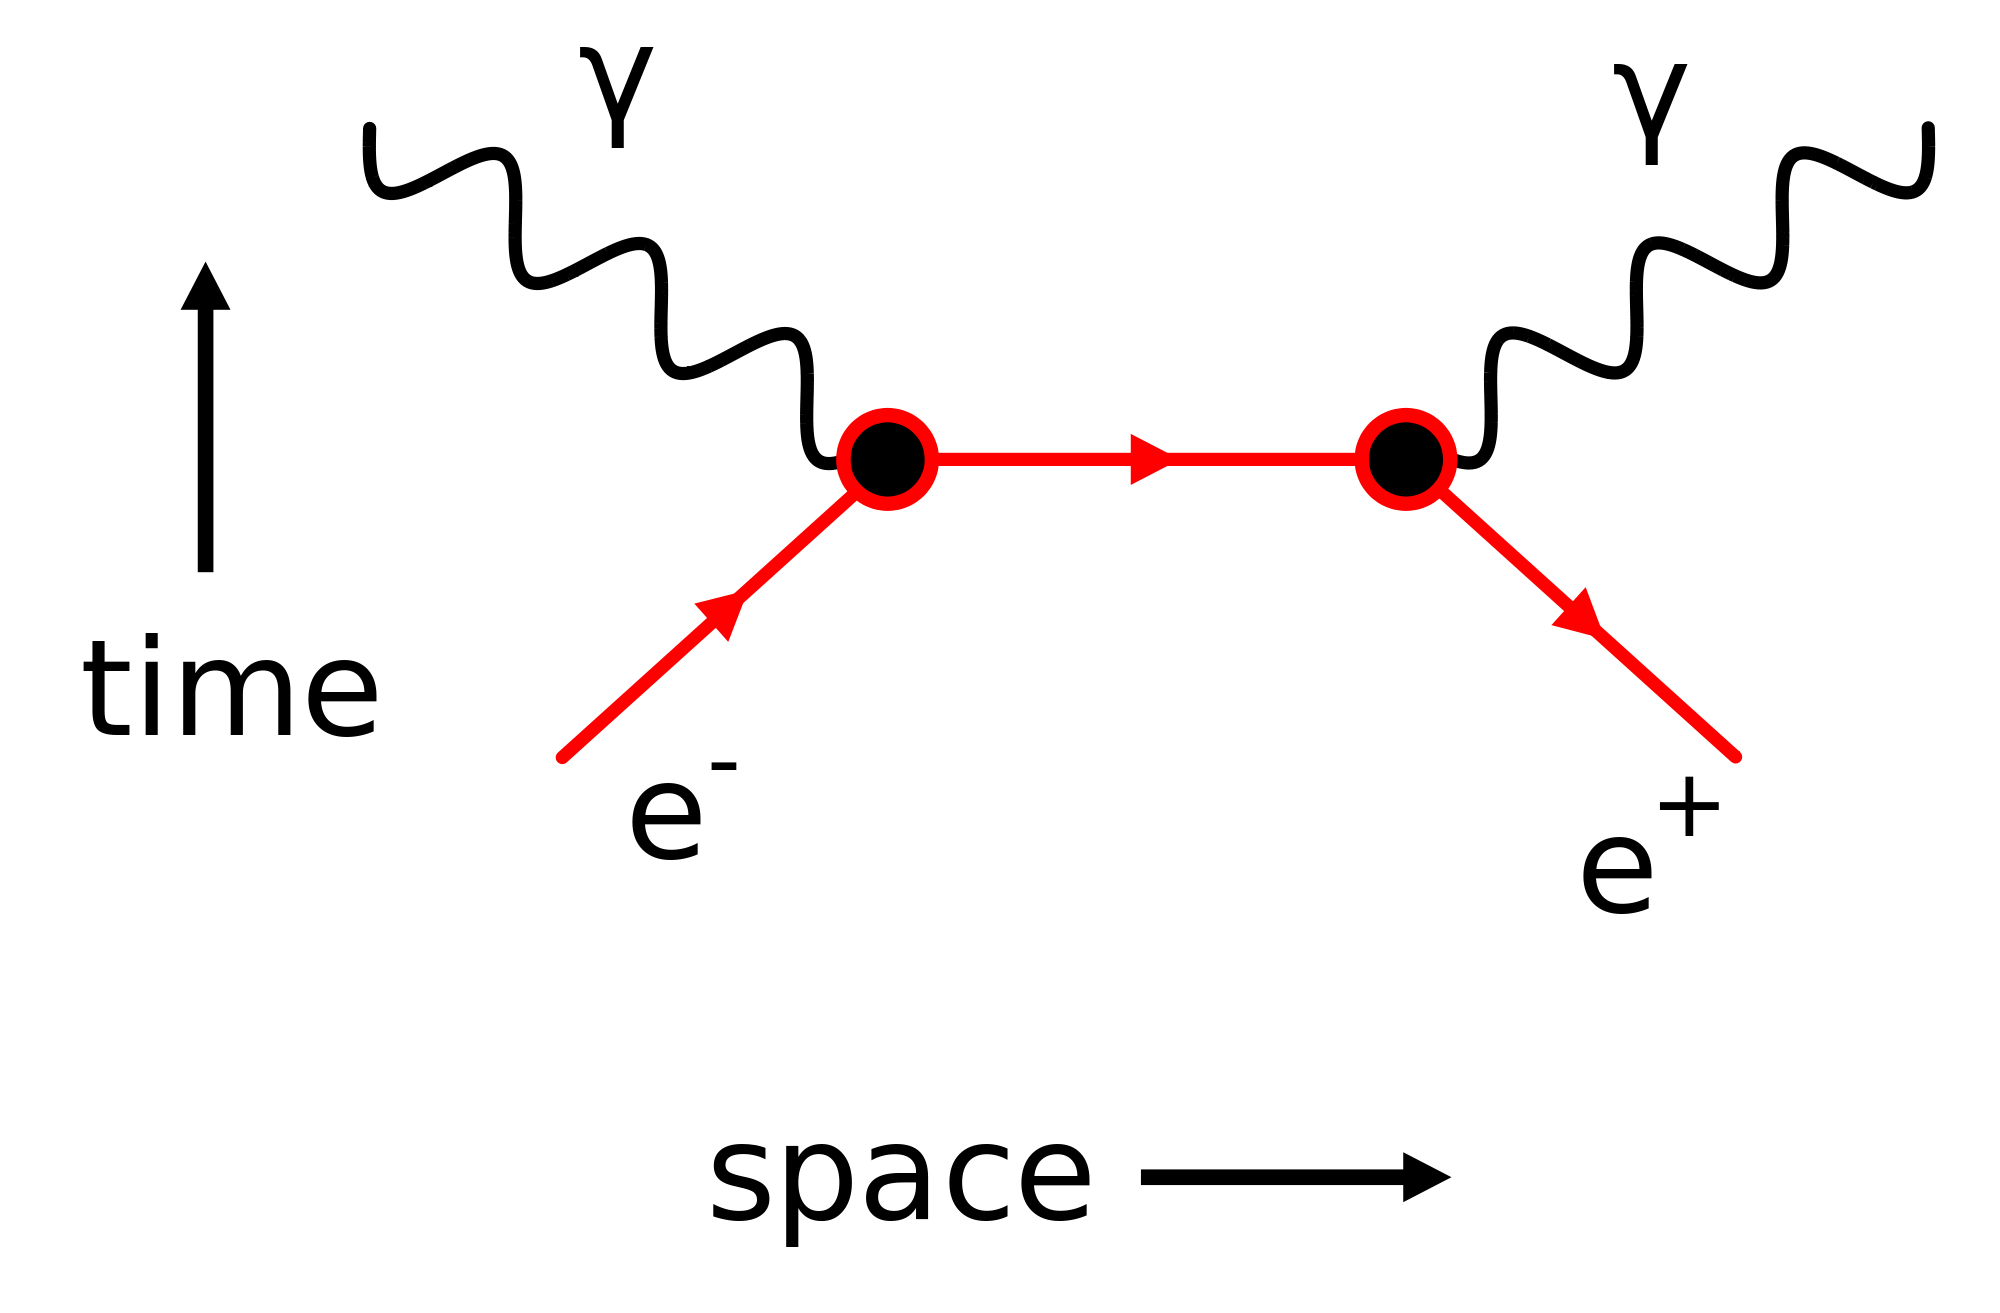
\includegraphics[scale = 0.08]{Bajas-energias.png}
            \caption{Diagrama de Feynman que representa la aniquilaci\'on electr\'on-positr\'on en dos fotones.}
            \label{fig:A-par-feynman}
        \end{figure}
\end{frame}

%%%%%%%%%%%%%%%%%%%%%%%%%%%%%%%%%%%%

\begin{frame}{Colisi\'on a altas energ\'ias}
    Si el electr\'on o el positr\'on, o ambos, tienen energ\'ia cin\'etica apreciable otras part\'iculas pesadas pueden ser producidas. \\
    \vfill
    \begin{figure}
        \centering
        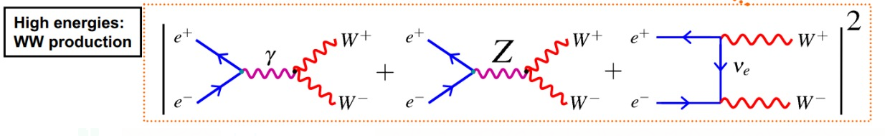
\includegraphics[scale = 0.5]{ColisionAEnergy.PNG}
        \caption{Diagrama de Feynman que representa una colisi\'on a altas energias.}
        \label{fig:Feynman-altasE}
    \end{figure}

\end{frame}
%que onda cara de verga
% kp2 pinchi putita
% mlp, quien quiera que seas 
%%%%%%%%%%%%%%%%%%%%%%%%%%%%%%%%%%%

\begin{frame}{Protón-antiprotrón}
En este caso, cuando ambos chocan con bajas energías no es necesario que el resultado sea pura energía (fotones) sino que a bajas energías suele involucrar la creación de mesones, los cuales eventualmente terminarán decayendo en neutrinos, fotones, electrones y positrones.
\par
Esto pasa de manera más general para cualquier interacción de baryon antibaryon(número impar de quark´s de valencia).
    
\end{frame}
%%%%%%%%%%%%%%%%%%%%%%%%%%%%%%%%%
% \begin{frame}{Creación de Higgs}
%     Los bossones de Higgs fueron descubiertos al hacer coliciones de protón-protón 
% \end{frame}
%%%%%%%%%%%%%%%%%%%%%%%%%%%%%%%%%
\section{Radiaci\'on de Hawking}
\begin{frame}{Radiación de Hawking}
    Stephen Haking postuló la existencia de este fenómeno en 1974, fenómeno de naturaleza cuántica ya que su origen cae en el principio de incertidumbre de Heisemberg.
    \par
    Gracias a este fenómeno se crean pares de partículas virtuales cerca del horizonte de eventos del agujero negro, donde una cantidad de partículas-antipartículas caen al agujero negro y otras no, dando origen a la creación de fotones vease, radiación.
    \begin{figure}[h]
        \centering
        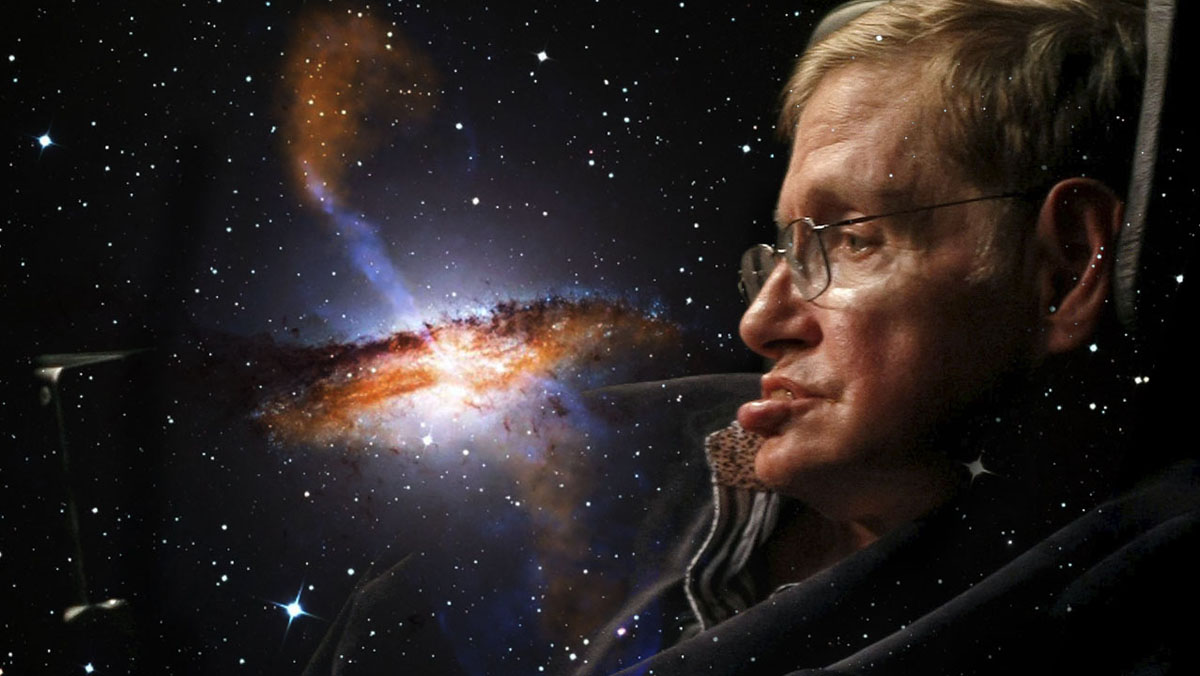
\includegraphics[scale = 0.13]{Estefano.jpg}
        \caption{Stephen Hawking}
        \label{fig:Estefano}
    \end{figure}
   
\end{frame}
%%%%%%%%%%%%%%%%%%%%%%%%%%%%%%%%%%
\begin{frame}{}
     \begin{figure}[h]
        \centering
        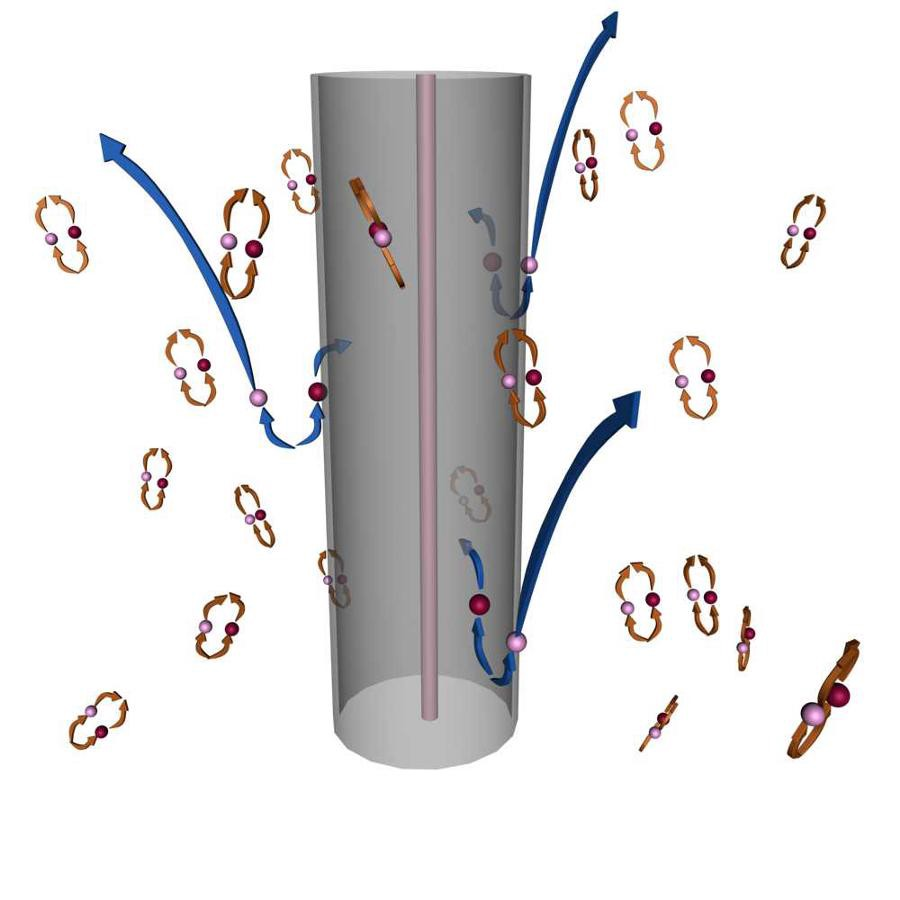
\includegraphics[scale = 0.23]{Creacion.jpeg}
        \caption{Ejemplo muy sencillo de partículas que parecen ser creadas de la nada}
        \label{fig:Creacion}
    \end{figure}
\end{frame}

%%%%%%%%%%%%%%%%%%%%%%%%%%%%%%%%%%
\begin{frame}{Temperatura de la radiación del agujero negro}
    \begin{equation*}
    \begin{split}
        & T=\frac{\hbar c^3}{8 \pi GMk_B} \left( \approx \frac{1.227\times 10^{23}kg}{M}K\right) \\
        & \hbar = \text{consante reducida de Planck} \\
        & c = \text{velocidad de la luz} \\
        & k_B = \text{constante de Boltzman} \\
        & G = \text{constante gravitacional} \\
        & M = \text{masa del agujero} negro 
    \end{split}
\end{equation*}
\end{frame}
%%%%%%%%%%%%%%%%%%%%%%%%%%%%%%%%%%
\begin{frame}{}
    \begin{figure}[h]
        \centering
        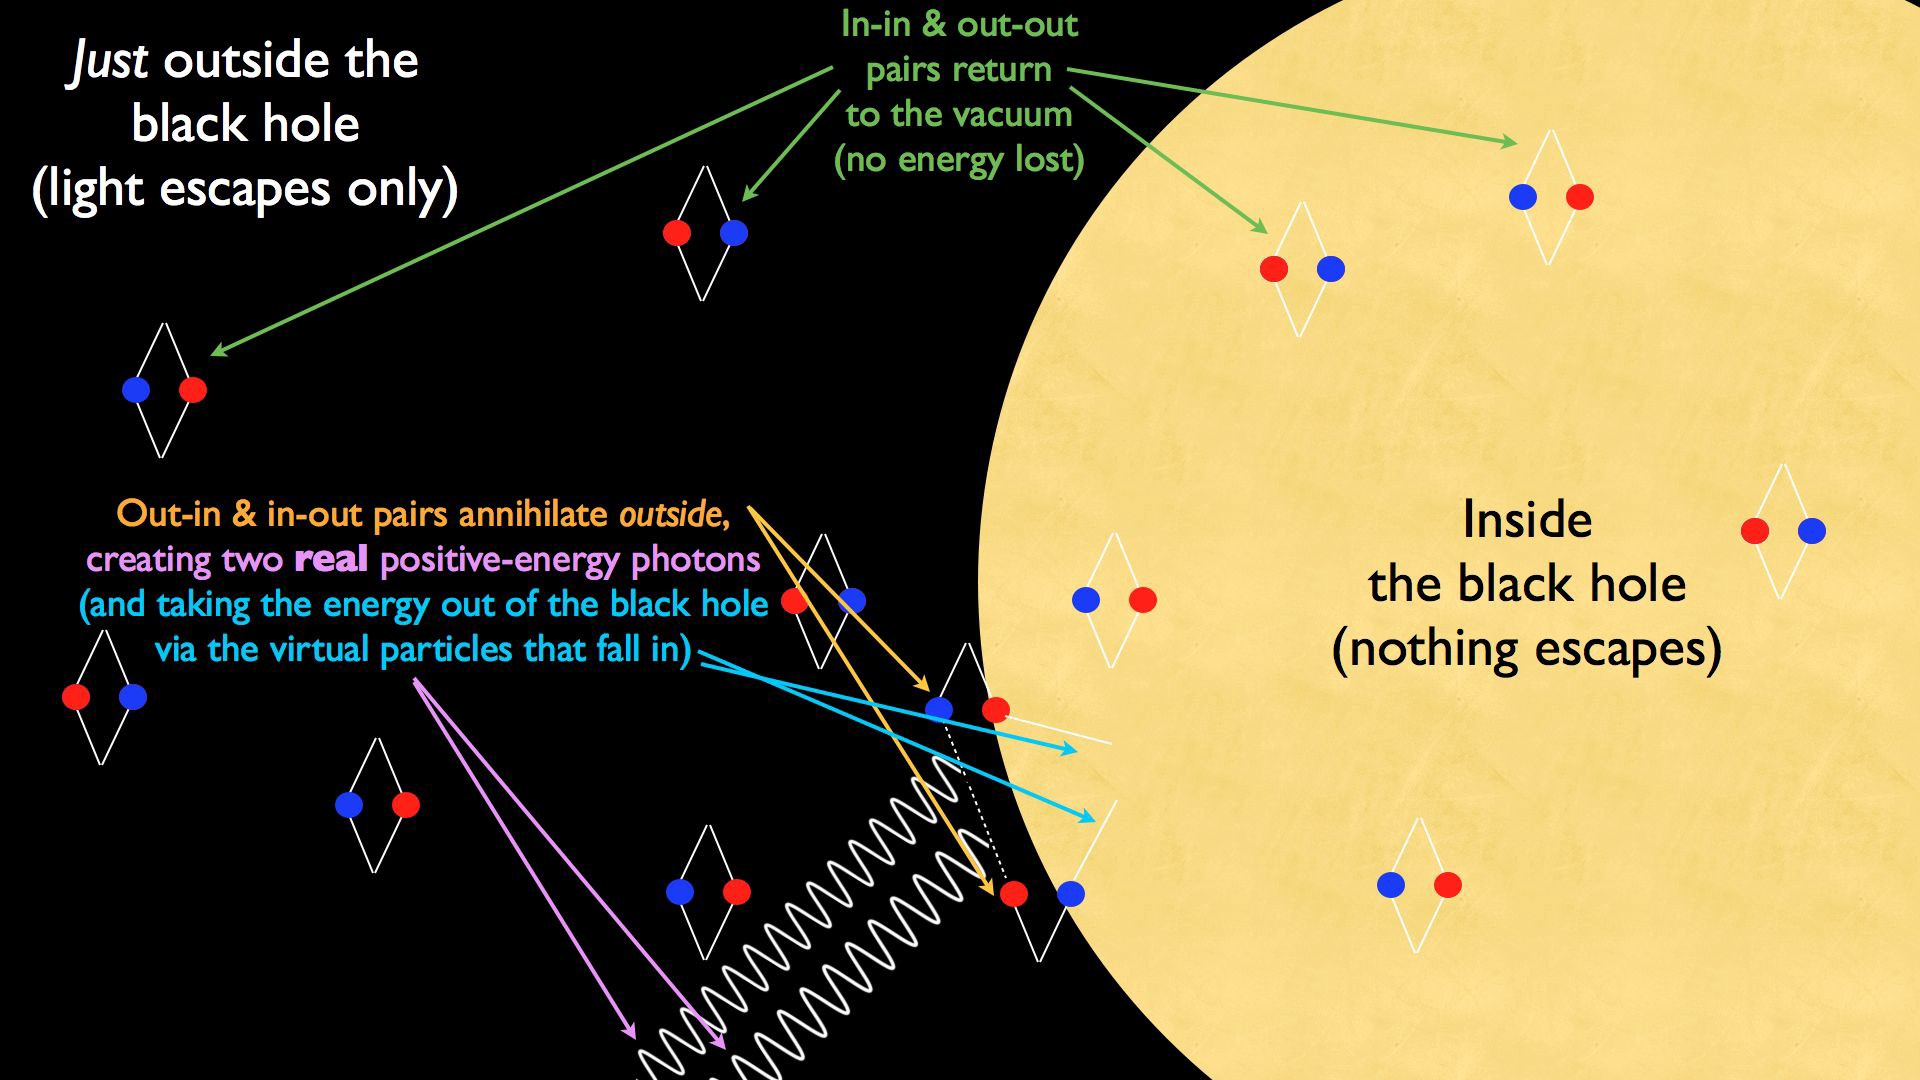
\includegraphics[scale = 0.17]{Rashos.jpeg}
        \caption{Simplificación de la radiación de Hawking}
        \label{fig:Rasho}
    \end{figure}
\end{frame}
%%%%%%%%%%%%%%%%%%%%%%%%%%%%%%%%%
\section{Conclusión}
\begin{frame}{Aplicaciones}


\begin{columns}
\begin{column}{.3\linewidth}\centering
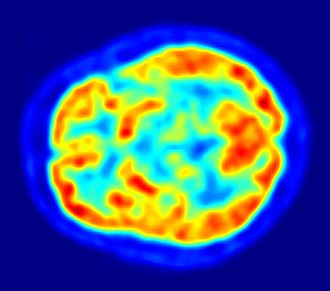
\includegraphics[width=\linewidth]{pet1.jpg}\par 

\end{column}
\begin{column}{.3\linewidth}\centering
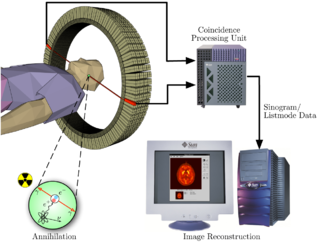
\includegraphics[width=\linewidth]{pet2.png}\par 
\end{column}
\begin{column}{.3\linewidth}\centering
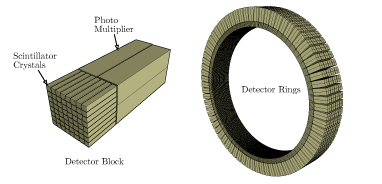
\includegraphics[width=\linewidth]{pet3.png}\par 

\end{column}
\end{columns}
\bigskip
Imagen de la actividad cerebral construída a partir de positrones interactuando con los electrones del cerebro.
\end{frame}
%%%%%%%%%%%%%%%%%%%%%%%%%%%%%%%%%

\begin{frame}{Aplicaciones}
\begin{figure}
    \centering
    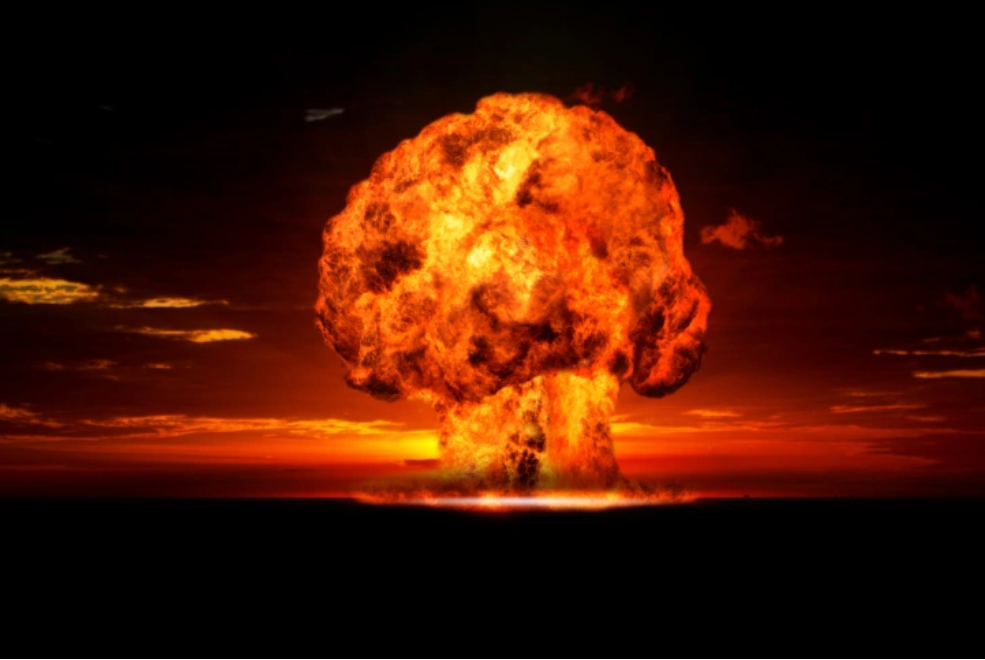
\includegraphics[scale=.4]{bomba.png}
    \caption{Una de las aplicaciones más controversiales.}
    \label{fig:my_label}
\end{figure}

\end{frame}

\begin{frame}{Aplicaciones}
\begin{figure}
    \centering
    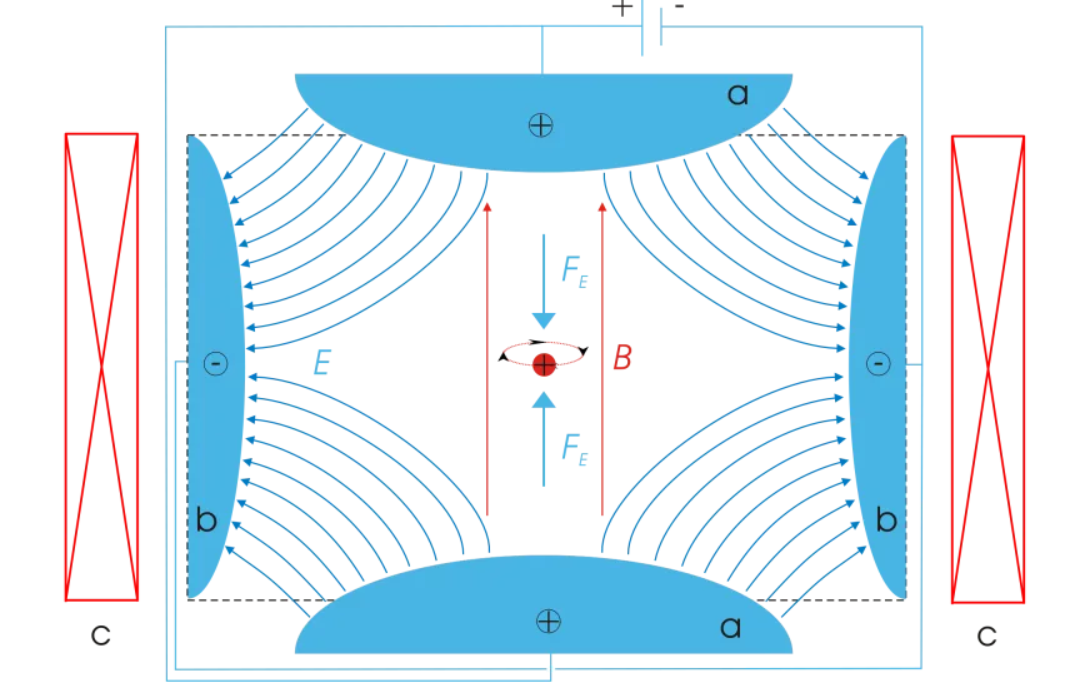
\includegraphics[scale=.4]{ion.png}
    \caption{Trampa iónica para almacenar antimateria.}
    \label{fig:my_label}
\end{figure}
    
\end{frame}


%%%%%%%%%%%%%%%%%%%%%%%%%%%%%%%%%
\begin{frame}{Problema}
    \textbf{ Un fot\'on $\gamma$ de 5 MeV genera un par electr\'on-positr\'on en las proximidades de un n\'ucleo pesado, inicialmente en reposo. Suponiendo que estas part\'iculas se reparten por igual la energ\'ia, calc\'ulese la energ\'ia cin\'etica del par part\'icula-antipart\'icula y su velocidad. }
    
    Para calcular la energ\'ia cin\'etica se tomar\'a en cuenta que la energ\'ia del fot\'on es igual a la suma de las energ\'ias del electr\'on y del positr\'on.
    \begin{equation*}
        \begin{split}
            E &= E_{-} + E_{+}\\
            E &= (m_0c^2 + k_{+}) + (m_0c^2 + k_{-})\\
        \end{split}
    \end{equation*}
    Como $k_{+} = k_{-}$
    $$ E = 2k + 2m_0c^2 $$
    De esta expresi\'on deduciomos el valor de la energ\'ia cin\'etica:
    $$ k = \frac{E - 2m_0c^2}{2} = \frac{2MeV - 1.022MeV}{2} = 1.99MeV $$
    \end{frame}

    \begin{frame}{}
        Ahora para obtener la velocidad.
        \begin{equation}\label{eq:Energia}
            E^2 = p^2c^2 + m_0^2c^4
        \end{equation}
        \begin{equation}\label{eq:momento}
            p = \frac{m_0v}{\sqrt{1-(v/c)^2}}
        \end{equation}
        Sustituyendo \eqref{eq:momento} en \eqref{eq:Energia}
        \begin{equation*}
            E^2 = \frac{m_062v^2c^2}{1-(v/c)^2} + m_0^2c^4
        \end{equation*}
        De aqu\'i podemo obtener la ecuaci\'on para la velocidad:
        \begin{equation}
            v = \frac{c}{E}\sqrt{E^2 - m_0^2c^4}
        \end{equation}
        Sustituyendo los datos:
        \begin{equation*}
            v = \frac{c}{2.50MeV}\sqrt{(2.50MeV)^2 - (0.511MeV)^2} = 0.98c
        \end{equation*}
    \end{frame}
%%%%%%%%%%%%%%%%%%%%%%%%%%%%%%%%%%
\begin{frame}{Conclusión}
¡Gracias kiks!
    \begin{figure}[h]
    \centering
    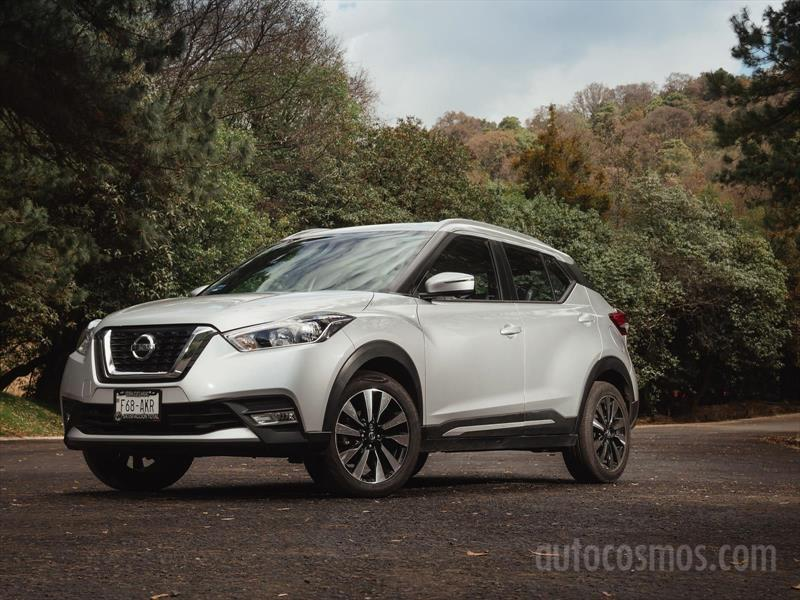
\includegraphics[scale = 0.35]{Kicks.jpg}
    \caption{Nissan Kicks}
    \label{fig:Kicks}
\end{figure}
\end{frame}
%%%%%%%%%%%%%%%%%%%%%%%%%%%%%%%%%%
%%%%%%%%%%%%%%%%%%%%%%%%%%%%%%%%%%
\section{Bibliografía}
%%%%%%%%%%%%%%%%%%%%%%%%%%%%%%%%%%
\begin{frame}{Bibliografía}
\begin{itemize}
    \item \textit{\textbf{Principio de incertidumbre de Heisemberg}} https://www.nucleares.unam.mx/~vieyra/node20.html
    \item \textit{\textbf{How do Black Holes evaporate?}} https://medium.com/starts-with-a-bang/how-do-black-holes-evaporate-5463dbda6832
    \item \textit{\textbf{Quantum fluctuation}} https://en.wikipedia.org/wiki/Quantum\_fluctuation
    \item \textit{\textbf{Uncertainty principle}} https://en.wikipedia.org/wiki/Uncertainty\_principle
    \item \textit{\textbf{What happens when a proton and an antiproton collide?}} https://www.quora.com/What-happens-when-a-proton-and-an-antiproton-collide
    \item \textit{\textbf{CERN}} 
    \par https://home.cern/
    \item \textit{\textbf{Annihilation}} 
    \par https://en.wikipedia.org/wiki/Annihilation
\end{itemize}
\end{frame}
\begin{frame}{}
    \begin{itemize}
        \item \textit{\textbf{Introduction to Nuclear and Particle Physics}}, Second Edition, A. Das and T. Ferbel, https://forum.lawebdefisica.com/entries/593-Imposibilidad-de-la-creación-de-pares-electrón---positrón-en-el-vacío
        \item \textit{\textbf{Imposibilidad de la creación de pares electrón-positrón en el vacío}} https://forum.lawebdefisica.com/entries/593-Imposibilidad-de-la-creación-de-pares-electrón---positrón-en-el-vacío 
        \item \textit{\textbf{Paul Dirac}} \par  https://es.wikipedia.org/wiki/Paul\_Dirac
        \item \textit{\textbf{Carl David Anderson}} https://es.wikipedia.org/wiki/Carl\_David\_Anderson
        \item \textit{\textbf{Cámara de niebla}} \par
        https://es.wikipedia.org/wiki/Cámara\_de\_niebla
        \item \textit{\textbf{Ejercicio}} \par
        https://www.eweb.unex.es/eweb/fisteor/andres/fisica\_cuantica/2010-2011/ejercicio1\_6.pdf
    \end{itemize}
\end{frame}
%%%%%%%%%%%%%%%%

%%%%%%%%%%%%%%%%

%melapelas

%%%%%%%%%%%%%%%%%%%%%%%%%%%%%%%%%%%%
% \section{How it Works}

% \begin{frame}{Yes Bank and NSDL}

% \begin{itemize}
%   \item Yes Bank is a depository participant of NSDL.

%   \item Yes Bank act as a middle man in the process of online tax payment.

% \end{itemize}

% \vskip 1cm
% \end{frame}

% \begin{frame}{NSDL}

% \begin{itemize}
%   \item NSDL is promoted byIndustrial Development Bank of India Limited(IDBI) - the largest development bank of India.
% \item NSDLis an Indian central securities depository.

% \end{itemize}
% \vskip 1cm

% \end{frame}


% %%%%%%%%%%%%%%%%

% \section{Benefits}

% \begin{frame}{Benefits}

% \begin{block}{From customer’s point of view}
% \end{block}
% \begin{itemize}

% %\end{}{itemize}
% \item Ease of access : Tax payers can track online the status of their challans deposited in banks
% \item Secure
%   \item Check present status of challan
%   \item Get Confirmation

% \end{itemize}

% \begin{block}{From Bank’s point of view}
% \end{block}
% \begin{itemize}

% %\end{}{itemize}
% \item Provide multiple services
% \item Make Business
% \item Increase Brand Value
% \end{itemize}

% \vskip 1cm
% \end{frame}

% %---------------------
% \section{References}
% \begin{frame}
% \frametitle{References}
% \begin{itemize}
% \item \url{https://nsdl.co.in/about/why.php/}
% \item \url{http://deic.uab.es/~iblanes/beamer_gallery/} \\
% \item \url{http://www.idbi.com/online-tax-payment.asp} \\
% \end{itemize}


% \begin{block}{E-Books}
% \begin{itemize}

% %\end{}{itemize}
% \item Programming ASP.NET 3.5 
% \item The Indian Financial System: Markets, Institutions and Services
% \end{itemize}
% \end{block}
% \vskip 1cm
% \end{frame}


% \section{End of Presentation}
% \begin{frame}
% \begin{itemize}[<+-| alert@+>]
% \item Thank You.
% \end{itemize}
% \end{frame}

\end{document}
